\newcommand{\texCommand}[1]{\texttt{\textbackslash{#1}}}%

\newcommand{\exemplo}[1]{%
\vspace{\baselineskip}%
\noindent\fbox{\begin{minipage}{\textwidth}#1\end{minipage}}%
\\\vspace{\baselineskip}}%

\newcommand{\exemploVerbatim}[1]{%
\vspace{\baselineskip}%
\noindent\fbox{\begin{minipage}{\textwidth}%
#1\end{minipage}}%
\\\vspace{\baselineskip}}%


\label{chap:ava}
\textbf{--> TRAZER o decreto de 2017 que define o que é EAD.}
Segundo Silva~\cite{silva2003educacao}, é imprescindível que se faça a distinção entre a educação puramente ``a distância'' e a educação on-line\footnote{Interação em tempo real, através de conexão na rede mundial de computadores.}: 

\begin{quote}
A modalidade “a distância”, via meios unidirecionais, separa emissão e recepção no tempo e no espaço. A modalidade online conecta professores e alunos nos tempos síncrono e assíncrono, dispensa o espaço físico, favorece a convergência de mídias e contempla bidirecionalidade, multidirecionalidade, estar-junto “virtual” em rede e colaboração todos-todos.
\end{quote}

Tendo em vista que esse trabalho se restringe às tecnologias utilizadas nessa dinâmica online de realizar EAD, este capítulo apresenta conceitualmente ao leitor o  \acrfull{AVA}, descrevendo seus aspectos tecnológicos e particularidades\textbf{ (FALAS de particularidades mesmo? Não seriam características?)}. Ainda busca apoiar o entendimento das funcionalidades de aprendizagem e das funcionalidades de avaliação disponíveis nesses ambientes, complementando e encerrando a fundamentação teórica desse trabalho. 
%%%%%%%%%%%%%%%%%%%%%%%%%%%%%%%%%%%%%%%%%%%%%%%%%%%
%%%%%%%%%%%%%%%%%%%%%%%%%%%%%%%%%%%%%%%%%%%%%%%%%%%
%%%%%%%%%%%%%%%%%%%%%%%%%%%%%%%%%%%%%%%%%%%%%%%%%%%
%%%%%%%%%%%%%%%%%%%%%%%%%%%%%%%%%%%%%%%%%%%%%%%%%%%
\section{O Ambiente, a Virtualização e a Aprendizagem}%

É possível categorizarmos a EAD, ao longo de sua trajetória histórica, em termos de estágios de evoluções tecnológicas acessíveis para serem empregadas na sua prática~\cite{dotta@ead}. Este histórico, define como a  primeira geração aquela que realizava a prática de instrução por meio de correspondência; a segunda geração que baseava o processo de ensino e aprendizagem a partir da transmissão de rádio e televisão;e, a terceira geração foi caracterizada pelo uso combinado das tecnologias de primeira e segunda gerações, agregando formas mais elaboradas de ensinos, tais como guias impressos e conferências por telefone. A quarta geração se destacou por incorporar tecnologias de interação em tempo real, através de áudio e videoconferência. Já, a geração atual é tida como a quinta geração, organizada em plataformas que reúnem vários recursos de interação online, com classes virtuais e operando por meio da infraestrutura de internet. \textbf{(--> ESTA CATEGORIZAÇÃO por gerações foi definida pelo autor [16]?}
\begin{figure}[h]
    \centering
    \smartdiagramset{
        set color list={cyan!10, cyan!20,cyan!30,cyan!40,cyan!50},
        sequence item font size=\footnotesize\sffamily,
        sequence item border size=1.2\pgflinewidth,        
    }    
    \smartdiagram[sequence diagram]{
      {1\textsuperscript{\underline{a}} geração\\instrução por correios},
      {2\textsuperscript{\underline{a}} geração\\rádio e televisão},
      {3\textsuperscript{\underline{a}} geração\\ correios, rádio e TV},
      {4\textsuperscript{\underline{a}} geração\\ conferência áudio-vídeo},
      {5\textsuperscript{\underline{a}} geração\\ plataformas online}}
    \caption{Gerações de tecnologias de Educação a Distância.}
    \label{fig:geracao}
\end{figure}      
  
  \textbf{--> NÃO utilizar acima e abaixo no texto, pois com as quebras de página esta referência pode se perder.}
Tomando como base a definição de educação online juntamente com a classificação da quinta geração de EAD, encontramos o nicho de aplicação de um \acrlong{AVA}. Doravante, sempre que a palavra EAD for utilizada será nessa conjuntura.

Troncon~\cite{RMRP86614} explica que o ambiente educacional pode ser entendido como ``todo e qualquer contexto em que se dá o ensino e o aprendizado'', e descreve elementos materiais (mobiliário, temperatura, iluminação, etc.) e elementos afetivos (senso de pertencimento, segurança, respeito, etc.) relacionados à ele. Nesse contexto, o significado da palavra \textbf{ambiente} serve para designar tanto o ambiente educacional quanto o ambiente computacional pelo qual se disponibiliza o ensino. Em EAD, uma parte dos elementos são delegados às condições do ambiente de acesso de cada aluno e, a outra, ao ambiente computacional intermediário do AVA\textbf{ (--> O QUE é ambiente intermediário do AVA?)}. 

A introdução do ambiente computacional adiciona novos aspectos na equação, apontados genericamente como aspectos do ambiente~\cite{Ferreira2016}. Dentre eles, podemos destacar a preocupação em apresentar um modelo de interface\footnote{Descreve como as informações são apresentadas na tela do usuário.} desenhado para melhorar a experiência do usuário; o esforço em estabelecer a não interrupção do serviço, através de medidas de contingência; o dimensionamento correto dos recursos computacionais necessários para entregar um ambiente com eficiência de velocidade e processamento; e a capacidade de integração com aplicações de terceiros. \textbf{--> NA NOTA de rodapé, tens que identificar a fonte desta definição.}

Seguindo para a palavra \textbf{virtual}, aqui é preciso que se tenha um certo cuidado para não haver confusão no seu emprego dentro do contexto educacional. Um ambiente de jogo recreativo, por exemplo, pode simular uma situação de fantasia ou ficção, e a palavra virtual pode ser empregada para descrever um cenário hipotético em oposição à uma situação real. Por outro lado, não é o que acontece quando uma pessoa usa a internet para se candidatar a uma vaga de emprego. Nesse segundo cenário, temos uma situação virtual em oposição à uma situação física de preencher um formulário. Embora o processo seja intermediado por meio digital, trata-se da recriação de um evento real no cotidiano de um cidadão. \textbf{--> E QUAL a definição do termo que será considerada neste trabalho? Tens que especificar.}

A virtualização tem a capacidade de expandir as propriedades das circunstâncias como as conhecemos, muitas vezes para fora das fronteiras do que entendemos como realidade, causando certos equívocos na concepção do que é virtual. Para exemplificar, dizemos que a educação semipresencial\footnote{Refere-se ao ensino híbrido de educação presencial e educação a distância.} combina aulas presenciais e virtuais, porém ambas são situações reais. Mesmo que a aula virtual tenha recursos não disponíveis em um contexto presencial, como a função pausa e a função retroceder, ainda estamos diante de uma realidade. Esse entendimento será necessário mais adiante para compreendermos a composição teórica das ferramentas presentes nesses ambientes.

Já pela escolha da palavra \textbf{aprendizagem}, percebe-se a preocupação é a de reafirmar o compromisso pedagógico com o desenvolvimento do discente. Ainda que hajam necessidades econômicas e estruturais impulsionando a EAD, o engajamento de docentes e discentes na construção da aprendizagem não foi omitido. A \refFig{fig:ava} ilustra os  relacionamentos desses três conceitos.
\begin{figure}[h]
    \centering
    \begin{tikzpicture}
      \begin{scope}[blend group = soft light]
        \fill[cyan!40, opacity=.4]   ( 90:1.2) circle (2);
        \fill[uclagold!40, opacity=.4] (210:1.2) circle (2);
        \fill[magenta!40, opacity=.4]  (330:1.2) circle (2);
        
      \end{scope}
      \node at ( 90:2)    {Aprendizagem};
      \node at ( 210:2)   {Ambiente};
      \node at ( 330:2)   {Virtual};
      \node [font=\Large] {AVA};
    \end{tikzpicture}
    \caption{Diagrama de conceitos de um AVA.}
    \label{fig:ava}
\end{figure}  

Além de comportar todos os conceitos descritos até aqui, ainda podemos adicionar que um AVA é um conjunto de funcionalidades, em que a maior parte delas está  voltada para a comunicação e para a troca de informações, fazendo dele uma solução colaborativa (groupware), apoiada no trabalho coletivo e no ambiente compartilhado. Para Oliveira \textit{et al.}~\cite{dotta@ead}, essa gama de recursos de interação traduz a importância de um AVA. Segundo os autores, a distância a ser vencida na EAD está além da simples separação física dos participantes, pois a aprendizagem precisa também vencer a barreira da distância transacional, causada por ausência de diálogo, rigidez na estrutura de ensino e a supressão da autonomia do aluno. Para os autores, essa distância transacional entre docentes e discentes pode ser percebida ``tanto no ensino presencial como a distância''. Ou seja, o auxílio de um AVA rico em possibilidades de interação não garante a aprendizagem em EAD se ele estiver sendo subutilizado pelos seus participantes.

Seguindo essa reflexão, podemos igualmente suspeitar que a prática da avaliação nesses ambientes também depende da redução dessa distância transacional. Não é difícil perceber, por exemplo, que a falta de capacitação da equipe multidisciplinar\footnote{Formada por professores, tutores, monitores e apoio técnico ao usuário} poderia impossibilitar o uso das funcionalidades que permitiriam a prática avaliativa. Ou, que um projeto pedagógico de EAD elaborado sem estratégias de interação, poderia prejudicar a tentativa de se realizar uma avaliação formativa, por exemplo.

Antes de partir para uma discussão de como mitigar os riscos mencionados, temos a necessidade de nos apropriar sobre essas funcionalidades e compreender como elas se relacionam com a avaliação da aprendizagem.

%%%%%%%%%%%%%%%%%%%%%%%%%%%%%%%%%%%%%%%%%%%%%%%%%%%
%%%%%%%%%%%%%%%%%%%%%%%%%%%%%%%%%%%%%%%%%%%%%%%%%%%
%%%%%%%%%%%%%%%%%%%%%%%%%%%%%%%%%%%%%%%%%%%%%%%%%%%
%%%%%%%%%%%%%%%%%%%%%%%%%%%%%%%%%%%%%%%%%%%%%%%%%%%

\section{Uma coleção de ferramentas e aplicativos}%

Funcionalidade, no contexto da engenharia de software, pode ser entendida como uma ação, criada para executar uma requisição do usuário. Assim, podemos dizer que a ação ``enviar mensagem'' é uma funcionalidade. O comportamento dessa ação é capturado pelo requisito funcional. Sommerville~\cite{sommerville2011eng} retrata um requisito funcional como aquele que ``descreve o que o sistema deve fazer''. 

Quando agrupamos diversas funcionalidades relacionadas entre si, em uma solução integrada, altamente especializada, temos um aplicativo~\cite{martins@tecnicas}. Seguindo o exemplo anterior, um aplicativo de correio eletrônico é composto de diversas funcionalidades, como enviar e receber mensagem, organizar pastas de mensagens, armazenar, dentre outras. Um agrupamento de aplicativos especializados em um único ambiente, costuma ser denominado como suíte ou pacote de aplicativos. Como exemplo, citamos a suíte Google Docs que contém aplicativos de planilhas, documentos, apresentações, formulários, e outros.

Uma Ferramenta também pode ser composta por uma ou mais funcionalidades relacionadas, porém não chega a ser tão especializado quanto um aplicativo, nem está disponível de forma avulsa. Uma ferramenta é um pedaço de um produto~\cite{martins@tecnicas} e só existe dentro dele. Como exemplo, podemos citar a Calculadora de um sistema operacional, pois o fabricante disponibiliza essa ferramenta para os usuários do sistema, mas não separadamente. Em geral, uma ferramente é parte de um sistema.

Do ponto de vista tecnológico, um AVA pode possuir tanto ferramentas próprias como ferramentas desenvolvidas por terceiros (third party), podendo ser integrado com aplicativos, suítes ou outros sistemas. Nesse caso, ele é considerado uma plataforma. Para fins desse estudo, o foco será mantido sobre o conjunto das ferramentas, mas alguns aplicativos serão mencionados com a finalidade de exemplificar situações ou, até mesmo, para sugerir substituições nos casos em que uma ferramenta equivalente não estiver na coleção. Ainda, sobre as características relativas a um AVA, Oliveira \textit{et al.}~\cite{dotta@ead} faz a seguinte distinção:

\begin{quote}
[...] ferramentas que exigem a participação simultânea de estudantes e professores em eventos marcados, com horários específicos (any place/real time), são classificadas como \textbf{síncronas}. As que independem de tempo e lugar (any place/any time) são classificadas como \textbf{assíncronas}. \textbf{(grifo nosso)}
\end{quote}

\textbf{--> QUEM PROPõS esta classificação? Não concordo e acredito que teremos diversos questionamentos neste sentido. Só porque o docente utiliza, não quer dizer que seja ferramenta de avaliação...}
Além dessa diferenciação em relação à sincronicidade, houve a necessidade de aplicar nesse levantamento a classificação de acordo com a finalidade do uso. Ou seja, as ferramentas voltadas para uso do discente serão denominadas de \textbf{ferramentas de aprendizagem}, e as que são utilizadas pela equipe docente de \textbf{ferramentas de avaliação}. A seguir, são apresentados os passos utilizados para a elaboração de uma listagem de ferramentas.

%%%%%%%%%%%%%%%%%%%%%%%%%%%%%%%%%%%%%%%%%%%%%%%%%%%
%%%%%%%%%%%%%%%%%%%%%%%%%%%%%%%%%%%%%%%%%%%%%%%%%%%
%%%%%%%%%%%%%%%%%%%%%%%%%%%%%%%%%%%%%%%%%%%%%%%%%%%
%%%%%%%%%%%%%%%%%%%%%%%%%%%%%%%%%%%%%%%%%%%%%%%%%%%

\subsection{Critérios de escolha das ferramentas}%
\textbf{--> PRECISAS ORGANIZAR ESTA SEÇÃO PARA O TEXTO ficar contínuo. Em escrita científica, não temos uma seção com apenas um parágrafo...}

\textbf{--> NAS NOTAS de rodapé onde explicas conceitos, precisas citar a fonte da definição. Precisa ter um autor para fazer a definição de um conceito... -- REVISAR todo o documento}
Embora seja possível para uma instituição demandar e desenvolver uma plataforma com recursos próprios, o custo e o tempo necessários para completar essa tarefa são vistos como desestimulantes, tornando mais vantajoso utilizar plataformas de código aberto\footnote{Modelo de licenciamento livre, em que qualquer pessoa pode examinar ou modificar o produto.} ou comerciais. Com base nesse entendimento, a seleção das ferramentas disponíveis em um AVA foi conduzida através de um levantamento exploratório em plataformas já estabelecidas na modalidade de EAD. A definição das duas plataformas utilizadas foi realizada com o auxílio da base de dados LISTedTECH\footnote{Banco de dados internacional de informações sobre empresas, produtos e instituições de EAD.}. 

Conforme dados do mês de  abril de 2018, fornecidos pelo relatório de cobertura da LISTedTECH~\cite{listedtech}, cerca de 50\% das 11.100 instituições de ensino superior que faziam parte da sua base utilizavam o Moodle como Ambiente Virtual de Aprendizagem. Em segundo lugar aparecia a plataforma Blackboard, com 19\%, seguida pela plataforma Canvas que aparecia com, aproximadamente, 12\% das instituições. O mapa de distribuição geográfica, apresentado pela organização, ainda informava que 437 instituições brasileiras faziam parte desse levantamento, porém, os dados não foram disponibilizados por região, sendo esses percentuais considerados os resultados globais de indicação de uso das plataformas.

A revista e-Literate\textbf{ (FAZER A REFERÊNCIA a revista)}, especializada em EAD, utilizou os dados da base LISTedTECH para apresentar uma análise das plataformas de acordo com a quantidade de vagas oferecidas pelas instituições~\cite{phil@lms}. O balanço foi apresentando em julho de 2017, e considerou a capacidade em três segmentos: pequeno (1 - 2.499 vagas), médio (2.500 - 14.999 vagas) e grande porte ($\geq$15.000 vagas). O estudo, que considerou dados da América do Norte e da Europa, possibilitou uma visão ponderada a respeito do uso dessas plataformas, diferenciando uma instituição com 1.000 vagas de uma com capacidade para 20.000, por exemplo. Esses números não refletem o número exato de matrículas, apenas utilizam a capacidade de vagas/alunos para estimar o potencial de matrículas disponíveis em EAD \textbf{(SEMIPRESENCIAL É CONSIderado EAD)}. 

Conforme a pesquisa realizada, o AVA mais utilizado por alunos na Europa foi o Moodle nos três segmentos, em segundo, o BlackBoard que foi listado em instituições de grande e médio porte, e o Canvas nas de pequeno porte. Já, na América do Norte, o Moodle é a primeira plataforma da maioria das instituições de pequeno porte, o BlackBoard nas de médio porte, e o Canvas aparece empatado com BlackBoard nas instituições de grande porte. A \refFig{fig:teste}. mostra a comparação ilustrativa das duas regiões e os percentuais de cada segmento.

\begin{figure}[h]
    \centering
    \fbox{    
        \begin{tikzpicture}
        
        \begin{groupplot}
          [
            group style=
            {
              group name=plataforms,
              group size=3 by 2,
              %horizontal sep=0pt,
              vertical sep=0pt,
              /pgf/bar width=15pt,
              xticklabels at=edge top,
              yticklabels at=edge left,
              xlabels at=edge bottom,
              ylabels at=edge left,
            },
          % limits settings
            xmin=0,
            xmax=0.8, 
            width=4.5cm,
            height=4.5cm,
            enlarge y limits=0.5,
            axis lines*=left,
            xbar,
          % axis lines
            axis x line=top,
            axis line style={-},
            y axis line style={opacity=0},
            major grid style={draw=gray},
          % labels
            symbolic y coords={{Pequeno}, {Médio}, {Grande}},
            ytick=data, %thanks to @Torbjørn T.
            ytick style={draw=none},
            ylabel style={align=center}, 
            xmajorgrids, 
            every axis x label/.style=
            {
              at={(rel axis cs:0.5,-.2)},
            },
          % ticks
            typeset ticklabels with strut,
            xtick distance = .2,
            tick align=inside,
          %nodes near coords
            nodes near coords={\tiny\pgfmathprintnumber\pgfplotspointmeta\%},
            nodes near coords style={fill=white},
            nodes near coords align={horizontal},
            point meta={x*100},
          ]
          \nextgroupplot[ylabel=Europa\\,]
            \addplot[draw=black,fill=uclagold] coordinates{(0.71,{Pequeno})  (0.58,{Médio}) (0.57,{Grande})};
          \nextgroupplot
            \addplot[draw=black,fill=forestgreen(web)] coordinates{(0.06,{Pequeno})  (0.17,{Médio}) (0.19,{Grande})};
          \nextgroupplot
            \addplot[draw=black,fill=purple] coordinates{(0.12,{Pequeno})  (0.04,{Médio}) (0.06,{Grande})};
            \label{Norte}
          \nextgroupplot[ylabel=America\\do Norte\\,xlabel=Moodle]
            \addplot[draw=black,fill=uclagold] coordinates{(0.37,{Pequeno})  (0.19,{Médio}) (0.09,{Grande})};
          \nextgroupplot[xlabel=BlackBoard,]
            \addplot[draw=black,fill=forestgreen(web)] coordinates{(0.18,{Pequeno})  (0.34,{Médio}) (0.33,{Grande})};
          \nextgroupplot[xlabel=Canvas,]
            \addplot[draw=black,fill=purple] coordinates{(0.17,{Pequeno})  (0.26,{Médio}) (0.33,{Grande})};  
          \end{groupplot}
        \end{tikzpicture}
    }
    \caption{Comparativo de plataformas de acordo com o porte institucional.}
    \label{fig:teste}
\end{figure}

\subsubsection{AVA por tempo de utilização}%

Ao longo do ciclo de vida\footnote{Termo absorvido da biologia para designar as adaptações e evoluções que asseguram a continuidade de um sistema.} de um sistema, os novos requisitos dos usuários são os responsáveis pelas principais evoluções nas suas ferramentas, ora adicionando ou evoluindo funcionalidades, ora descontinuando as que se tornaram desnecessárias. Se considerarmos essa informação, o tempo de distribuição das plataformas pode significar um maior amadurecimento das soluções de EAD. Neste sentido, identificou-se que o Moodle, iniciou em  2002, o BlackBoard Learn, em  2004, e o Canvas, em  2011.

Considerando os três critérios apresentados (quantidade de licenças, de vagas e tempo de atuação), definiu-se realizar o levantamento nas duas plataformas que mais se destacaram nestes itens. Para a realização do levantamento, foram utilizados os catálogos de divulgação de ferramentas de ambas as plataformas~\cite{moodle}~\cite{bblearn}, associados a técnicas de engenharia reversa\footnote{Observação das características e do comportamento de um produto final com a intenção de descobrir seu funcionamento e seus requisitos.}. A catalogação é apresentada em duas partes, conforme se segue:
\begin{enumerate}
	\item Ferramentas consideradas de ensino e auxílio à aprendizagem, foram designadas por um nome genérico e descritivo, seguido de um detalhamento de suas funcionalidades observáveis. Dessa forma, a ferramenta de visualização de terceiros ao vivo,  conhecida como \emph{BigBlueButton}, foi mesclada com as estatísticas de visualização de uma aula previamente gravada, disponibilizada na plataforma BlackBoard, foi identificada pelas designações genéricas de suas funcionalidade como ``Transmissão'' e ``Conferência''. E a descrição básica de suas funcionalidades, nos seus dois modos de uso, foram capturadas a partir de visualização de suas ações e características de interface. Essa descrição não teve a intenção de capturar completamente seu funcionamento, apenas aspectos gerais das suas finalidades. Essas ferramentas são descritas na Seção~\ref{sec:aprend}. \textbf{--> ESTA EXPLICAÇÃO está bastante confusa. Recomendo reescrever e ser mais direta.}
	\item As ferramentas consideradas de avaliação e acompanhamento seguiram a mesma designação genérica, porém, em alguns casos, foi utilizado o agrupamento de funcionalidade com mesma finalidade para denominar e descrever as ferramentas. Ou seja, a funcionalidade que mostra as estatísticas de visualização de uma aula ao vivo, disponibilizada via \emph{BigBlueButton}, foi mesclada com as estatísticas de visualização, disponibilizada por outra ferramente, das aulas previamente gravadas e publicadas para visualização assíncrona. Essa aglomeração gerou a ferramenta denominada ``Acompanhar aulas'' e a sua descrição funcional. A lista dessas ferramentas pode ser encontrada na Seção~\ref{sec:aval}. \textbf{--> ESTA EXPLICAÇÃO está bastante confusa. Recomendo reescrever e ser mais direta.}
\end{enumerate}
%%%%%%%%%%%%%%%%%%%%%%%%%%%%%%%%%%%%%%%%%%%%%%%%%%%
%%%%%%%%%%%%%%%%%%%%%%%%%%%%%%%%%%%%%%%%%%%%%%%%%%%
%%%%%%%%%%%%%%%%%%%%%%%%%%%%%%%%%%%%%%%%%%%%%%%%%%%
%%%%%%%%%%%%%%%%%%%%%%%%%%%%%%%%%%%%%%%%%%%%%%%%%%%
\section{Ferramentas de ensino e auxílio da aprendizagem}%
\label{sec:aprend}
\textbf{--> INSERIR itens em cada um dos tópicos. Nos texto temos ou tópicos ou títulos de seção. Neste caso, precisam ser itens (não numerados)}
\textbf{ANTES DE passar para a sub-seção (3.3.1, precisas ter um texto introdutório após o título da seção 3.3). Além disso, recomendo trazer as definições de cada um dos itens de um autor da área. É importante trabalhar com conteúdos que já estão formalizados na bibliografia. Podes fazer até a citação direta dos autores. REVISAR ESTA SEÇÃO}
\subsection{Assíncronas}%
\textbf{--> É PRECISO fazer uma introdução nesta sub-seção também. Falar o que representam estes itens.}
\begin{description}
\item[Painel de Informações:] local específico para formalizar o plano da disciplina, apresentar claramente quais são os pré-requisitos tecnológicos e de habilidades, os objetivos da aprendizagem, procedimentos e técnicas que serão utilizadas, e os critérios e objetos de avaliação. Algumas vezes essa área aparece no modo público, isto é, sem que haja a necessidade de se utilizar senhas para acessar a informação. \textbf{-->A INFORMAÇÃO DESTA ÚLTIMA FRASE É necessária para o trabalho? Acho que pode ser excluída.}
\item[Quadro de anúncios:] área de destaque utilizada pela equipe docente para manter os discentes atualizados sobre alterações importantes e informações a respeito do andamento do curso/disciplina. É importante que essas informações tenham um local específico e de destaque para não gerar confusão.
\item[Mensagem:] funcionalidade utilizada para comunicação direta entre dois ou mais membros. Pode ser no formato de correio, com funcionalidades de estilo de texto, ou de texto simples.
\item[Notificações:] funcionalidade responsável por realizar o serviço de notificações de eventos no ambiente. Por exemplo: adições de conteúdos, de notas, ocorrências de calendário, comentários em tarefas, dentre outros. É uma ferramenta essencial para manter os estudantes atualizados sobre os acontecimentos relacionados ao curso/disciplina.
\item[Mural:] área de compartilhamento de informação entre componentes da disciplina/curso. O intuito é incentivar o diálogo informal que aconteceria normalmente nos intervalos de uma aula presencial. Caso existam políticas de uso, devem estar visíveis.
\item[Fórum de discussões:] ferramenta utilizada para compartilhamento de questões gerais e específicas sobre assuntos relacionados estritamente ao curso/disciplina. Dúvidas sobre interpretações de uma tarefa, relatos de erro material do conteúdo e solicitações de interesse geral são exemplos de uso. Os fóruns simulam o diálogo que aconteceria naturalmente durante um encontro presencial de aula, quando um discente faz perguntas ou oferece observações na presença do docente.
\item[Calendário:] utilizado para agendamento e acompanhamento do cronograma das atividades do curso/disciplina. Registros de data e hora de ações avaliativas, de entrega de tarefas, de conferências agendadas são exemplos de atividades que devem constar na agenda. Serve para todos terem uma noção visual dos eventos e se programarem.
\item[Repositório:] área destinada para compartilhamento de conteúdos eletrônicos como planilhas, apresentações, documentos, páginas externas, pacotes de arquivos, etc. Informações textuais sobre a organização do repositório e os resumos dos assuntos devem estar disponíveis para auxiliar os membros a navegar pelos conteúdos.
\item[Wiki:] utilizada para construção de textos colaborativos. Podendo compreender assuntos relacionados ao curso/disciplina, desde de pré-requisitos até aprofundamentos de conteúdo. Dentro das páginas rápidas de consulta, cada conteúdo pode trazer um histórico com origem, exemplos de aplicação, imagens ilustrativas, e outras. Tem muita utilidade nos trabalhos em grupo.
\item[Glossário:] serve como lista de definições e conceitos. É uma ferramenta simples de disseminar informações de qualidade sobre definições importantes para compreensão dos assuntos do curso/disciplina.
\item[Mini-página:] é o local em que o aluno se apresenta, pode ter campos pré-definidos e abertos. Através da mini-página os membros podem conhecer melhor sobre informações básicas uns dos outros.
\item[Perguntas Frequentes:] compilação, normalmente feita pela equipe docente, das perguntas mais frequentes feitas à eles. É importante para reduzir o número de perguntas repetitivas e para que os membros do grupo se informem rapidamente. Precisa estar em um local de destaque. Normalmente os fóruns possuem avisos e apontamentos para as Perguntas Frequentes e solicitam que o membro faça uma consulta na lista antes de enviar uma nova postagem.
\item[Enquete:] utilizada pela equipe docente na realização de pesquisas de opiniões ou em qualquer situação que seja necessário os discentes decidirem sobre alguma coisa. A enquete é uma poderosa ferramenta de consulta, dando visibilidade e transparência sobre os resultados, além de auxiliar na participação do grupo e na autoafirmação individual. Pode ser utilizada para simular consultas que um docente faria em aulas presenciais.
\item[Aula multimídia:] área de compartilhamento de roteiros das aulas que foram transmitidas de forma síncrona ou, em caso de EAD híbrido, das aulas presenciais. São as notas e tópicos visuais que foram apresentados pelo docente em quadro negro ou com slides. As apresentações são importantes para os alunos revisitarem a aula, relembrarem o que aprenderam ou até mesmo descobrirem o que perderam, nos casos em que não puderam assistir. Também utilizada para compartilhar vídeo de aulas transmitidas que foram gravadas, ou que podem ter sido gravados e editados isoladamente com recursos de legendas, inclusão de telas de imagens, repetição de cenas, etc. A área de aula deve estar em formato sequencial, como uma linha do tempo do andamento do curso/disciplina.
\item[Tarefas:] local de entrega de tarefas com prazos definidos, utilizado para os alunos enviarem os resultados finalizados de trabalhos, exercícios realizados fora da plataforma, pacotes de documentos entregáveis como planilhas, arquivos de código, imagens ou modelos. 
\item[Questionário:] formulário de questões dirigidas aos alunos dentro da plataforma, pode ser usado como tarefa durante a aula ou em horários alternativos, podem ou não ter prazo de conclusão. Permite o uso de diferentes tipos de questões como as de verdadeiro/falso, perguntas com espaço em branco, mistura de palavras, listas de correspondência, lista de múltipla escolha e redação.  
\item[Simulados:] em geral é a mesma ferramenta utilizada para exames e testes, mas configurada para funcionar em modo assíncrono e sem prazo. Serve para que o aluno se familiarize com a ferramenta de testes, com os tipos de questões, nível de complexidade do exame. Ou seja, para ele conhecer o exame e tirar dúvidas pré-teste (ver Exame na Subseção~\ref{sub:sinc}).
\item[Painel de Controle:] importante ferramenta de configuração e customização. Um aluno com daltonismo pode utilizar a customização do ambiente para alterar as cores da forma mais confortável, por exemplo. Membros podem ajustar as notificações quanto ao meio de recebimento (correio eletrônico, painel de notificação, torpedos), e quanto aos seus conteúdos para restringir ou abranger a quantidade de avisos recebidos. É importante que notificações de publicações no Quadro de anúncios não possam ser completamente desabilitadas, por questões de segurança no processo de formalização.
\item[Quadro de notas:] quadro de acompanhamento do aluno, usado para dar visibilidade do andamento da avaliação realizada. O quadro ainda pode fornecer visões em gráficos, percentuais de avaliações participadas e perdidas, próximas avaliações, feedback das tarefas com observações sobre erros e pontos de inobservância ou de ajustes. O quadro da avaliação deve ser atualizado o mais rápido possível, permitindo que os alunos possam reagir e se autoajustar.
\item[Suporte:] ferramente de comunicação com a equipe de suporte técnico da plataforma, permitindo que os membros possam solicitar auxílio que dizem respeito aos aspectos tecnológicos, como perdas de senha, erros de navegação, incompatibilidades de aplicativos, etc.
%%%%%%%%%%%%%%%%%%%%%%%%%%%%%%%%%%%%%%%%%%%%%%%%%%%
%%%%%%%%%%%%%%%%%%%%%%%%%%%%%%%%%%%%%%%%%%%%%%%%%%%
%%%%%%%%%%%%%%%%%%%%%%%%%%%%%%%%%%%%%%%%%%%%%%%%%%%
%%%%%%%%%%%%%%%%%%%%%%%%%%%%%%%%%%%%%%%%%%%%%%%%%%%
\subsection{Síncronas}%
\label{sub:sinc}
\textbf{--> DA MESMA FORMA QUE O ANTERIOR, precisas trazer a definição dos itens baseando-se em um autor da área. Em documentos científicos, a apresentação de conceitos deve se basear em algum documento científico...}
\item[Transmissão multimídia:] a transmissão ao vivo pode ser feita por áudio, ou áudio e vídeo. Normalmente utilizadas para dar aulas em horários pré-definidos, marcados com antecedência. As transmissões podem ser usadas no formato de aulas regulares ou pontuais a distância, ou para realização de conteúdos extras para os quais não há aulas gravadas. Em algumas modalidades de EAD, a transmissão é feita com auxílio de equipamentos de alta qualidade para capturar as imagens em alta definição, sendo realizadas em salas específicas.
\item[Conferência:] a conferência é uma ferramente de reunião, muitas vezes é realizada na mesma ferramenta de transmissão, habilitando-se as duas vias de áudio (envio e resposta). Usada com frequência para realizar debates, promover momentos de interação, realizar dinâmicas de grupo e até mesmo exames orais.
\item[Bate-papo:] ferramente textual para comunicação síncrona, permite conversas individuais e coletivas, compartilhamento de arquivos e endereços da internet. Pode ser a mesma ferramente de troca de mensagens sendo utilizada de forma síncrona com marcação de hora para iniciar.
\item[Exame:] o exame on-line pode ser realizado com o auxílio de uma ferramenta configurada para ser habilitada durante um intervalo pré-definido de tempo e com hora marcada. A ferramenta possui funcionalidade que paralisam o teste se o foco do usuário sair da tela ou registrar momentos de inatividade. Pode ser configurado para capturar o áudio e o vídeo do aluno no momento do exame (o aluno precisa conceder o acesso). Pode ser realizado em uma máquina física instalada em ambiente restrito no local de domicílio do aluno.
\end{description}

Algumas ferramentas foram dispensadas por não apresentarem muita relação com as ferramentas de avaliação. Como exemplo, citamos a área de busca, marcadores de página e favoritos, dentre outras.
%%%%%%%%%%%%%%%%%%%%%%%%%%%%%%%%%%%%%%%%%%%%%%%%%%%
%%%%%%%%%%%%%%%%%%%%%%%%%%%%%%%%%%%%%%%%%%%%%%%%%%%
%%%%%%%%%%%%%%%%%%%%%%%%%%%%%%%%%%%%%%%%%%%%%%%%%%%
%%%%%%%%%%%%%%%%%%%%%%%%%%%%%%%%%%%%%%%%%%%%%%%%%%%
\section{Ferramentas de avaliação e acompanhamento}%
\label{sec:aval}
\begin{description}

\item[Gerenciamento de grupo:] criação e acompanhamento de grupos personalizados. O docente pode agrupar alunos para otimizar suas interações com os grupos formados no ambiente. Isso permite que ele envie a mesma mensagens ou um feedback para todos os integrantes de forma conjunta. Ou que acompanhe o desempenho das estatística e relatórios nas outras ferramentas pela visão dos grupos de trabalho ou do grupo inteiro. 

\item[Programação do curso:] permite montar o roteiro com todas as aulas e tarefas dentro de um cronograma sequencial, criando fluxos de ensino-aprendizagem para posterior acompanhamento do andamento dos membros de acordo com os marcos estabelecidos.

\item[Acompanhar anúncios:] exibe a lista dos alunos que visualizaram os anúncios de alteração publicados no Quadro de anúncios. Com o auxílio dessa ferramenta o docente pode identificar se todos estão cientes das mudanças no Plano da disciplina ou cancelamentos de aula, por exemplo. Permitindo ao docente atuar nessas questões. 

\item[Acompanhar notificações:] exibe a lista de notificações enviadas pela plataforma e relatório das que foram visualizadas. Permite também configurar quais notificações se deseja que a plataforma envie, customizar mensagens, reenviar notificações individuais ou coletivas.

\item[Recuperação de conteúdo:] exibe relatórios de conteúdos que foram acessados pelo grupo, com filtros de seleção de membros individuais ou grupos. Apresenta estatísticas de leitura, cobertura do conteúdo acessado, taxas de transmissão e volumetria de dados baixados. 

\item[Mapeamento de Competências:] análise de lacunas e de habilidades. Permite ao docente identificar dificuldades em pré-requisitos e potenciais alunos com condições de auxiliar no aprendizado deles.

\item[Acompanhar colaboração:] apresenta relatórios de tempo de uso, cliques, quantidade de mensagens enviadas através de cada ferramenta de comunicação, postagens em ferramentas colaborativas, dentre outras análises sobre a interação do aluno com o ambiente e com outros alunos. O gráfico de colaboração permite identificar grupos de colaboração e pontos de isolamento.

\item[Acompanhar dificuldades:] registras as interações dos alunos com a equipe de apoio como monitores, instrutores, suporte, acesso a ferramentas de ajuda. Identifica os alunos que possam precisar de algum tipo de atuação, pontos de melhoria no curso, média de tempo de resposta da equipe de apoio ou docente, e outros. 

\item[Acompanhar questionários:] a ferramenta de aplicação de questionários possui gabarito e pode realizar a correção automaticamente. Não obstante, o acompanhamento de questionário permite ao docente verificar quem respondeu; o tempo que levou para responder e a média do tempo da turma; as questões com maior índice de respostas erradas, ajudando a identificar possíveis problemas com o comando da questão ou com pré-requisitos; e relatórios de análise em geral.

\item[Revisão de textos:] auxília na correção de textos, permitindo análise de ortografia, concordância, plágio, contagem de plavras, revisão em pares, dentre outras.

\item[Acompanhar tarefas:] fornece relatórios de entregas e atrasos das tarefas, tentativas que resultaram em falhas e informação do erro, além de configuração dos parâmetros de entrega.

\item[Acompanhar aulas:] fornece estatísticas sobre as visualizações das transmissões on-line e das aulas gravadas, permitindo ao docente acompanhar o andamento da turma em relação ao conteúdo obrigatório.

\item[Acompanhar exames:] oferece informações em tempo real sobre o andamento do exame, permitindo ao docente acompanhar individualmente ou por grupos. 

\item[Registrar notas:] permite configurar o plano de avaliações, registrar as notas e enviar feedback das avaliações. As notas automaticamente apuradas podem ou não  ser confirmadas manualmente pelo docente antes de serem lançadas no quadro. A ferramenta deve permitir edições para correções de notas após o lançamento.

\item[Acompanhar quadro de notas e feedback:] permite ao docente verificar se os alunos estão acompanhando suas notas e as revisões e recomendações apontadas durante a avaliação.

\item[Orientação:] aceitar ou propor marcações de orientações através das ferramentas síncronas de comunicação. Configurar horários e datas de disponibilidade de orientações.

\end{description}

Algumas ferramentas foram dispensadas por não apresentarem funções de avaliação e sim de gerenciamento e administração. Como exemplo, citamos a configuração da quantidade de vagas, aceite de matrículas, cadastro da equipe, entre outras.

\section{Matriz de relacionamento entre ferramentas}
\textbf{--> APRESENTAR o conceito formal de matriz de relacionamento...}
Tendo em vista explicitar a relação entre as ferramentas de aprendizagem e as ferramentas de avaliação, criou-se a \refFig{fig:ferramentas}, onde podemos identificar quais ferramentas precisam estar habilitadas para uso dos usuários e da equipe, caso o docente deseje realizar alguma atividade de avaliação.
\textbf{--> NÃO FICOU claro como obtiveste esta matriz. Pecisas detalhar melhor para o que ela será utilizada.}

%\begin{landscape}

    \begin{figure}[h]
        \centering
            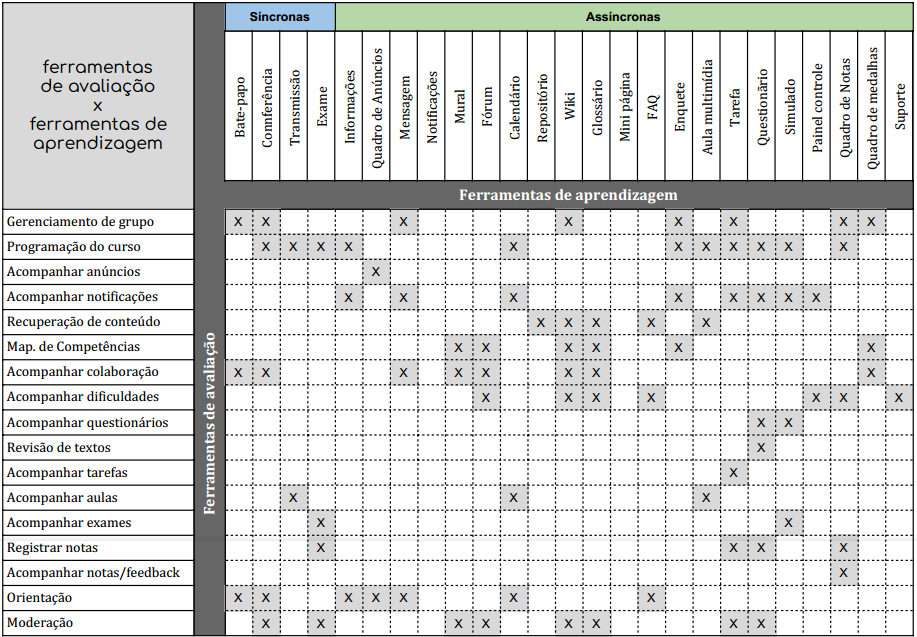
\includegraphics[width=\textwidth]{img/ferramentas_avaliacao.png}
        \caption{Matriz de vínculo entre ferramentas.}
        \label{fig:ferramentas}
    \end{figure}
%\end{landscape}

Para exemplificar, tomemos como premissa que um determinado docente deseje realizar a atividade de avaliação denominada como ``Acompanhar dificuldades'', na qual ele utiliza dados parametrizados fornecidos pelo sistema para identificar se os discentes estão encontrando obstáculos no uso da plataforma. Para realizar essa avaliação, esse docente precisaria ter uma ou mais dessas ferramentas habilitadas: Fórum, Wiki, Glossário, FAQ e/ou Suporte.

No caso em que esse mesmo docente não tenha habilitado nenhuma dessas ferramentas, a solução seria fazer um levantamento manual com a equipe para tentar identificar quais os problemas que os alunos mais reportaram. Ou, então, submeter algum tipo de consulta aos discentes para que esses informassem manualmente quais contratempos enfrentaram, tornando a atividade mais onerosa e passíveis de inconsistências. Neste exemplo, podemos perceber que a matriz pode ser útil no planejamento das ações avaliativas, por antecipar os requisitos necessários para realizar a avaliação. O levantamento descritivo das ferramentas, associado à matriz de vínculos, pode gerar um catálogo das funcionalidades capazes de subsidiar a prática da avaliação em um AVA. Ainda, pode-se identificar a vinculação de uma ação avaliativa com sua função de avaliação, relacionando a ação com a intenção. 